\documentclass[aspectratio=169]{beamer}
\setbeamertemplate{navigation symbols}{}
\usepackage{color,amsmath,comment, subfigure}
\usepackage{booktabs}
\usepackage{url}

%%%%%%%%%%%%%%%%%%%%%%%%%%
\title[]{Class 21: Fixing social media}
\author[]{Matthew J. Salganik}
\institute[]{Sociology 204: Social Networks\\Princeton University}
\date[]{
1/2 Background and context
\vfill

\begin{flushleft}
\vspace{0.6in}

\includegraphics[width=0.1\textwidth]{figures/cc.png}
\end{flushleft}
}

\begin{document}
%%%%%%%%%%%%%%%%%%%%%%%%%%%
\frame{\titlepage}
%%%%%%%%%%%%%%%%%%%%%%%%%%%
\begin{frame}

{\LARGE
\begin{center}
\only<1>{Fixing social media}%
\only<2>{``Fixing'' social media}%
\only<3>{Changing social media}%
\end{center}
}

\end{frame}
%%%%%%%%%%%%%%%%%%%%%%%%%%%
\begin{frame}

\begin{center}
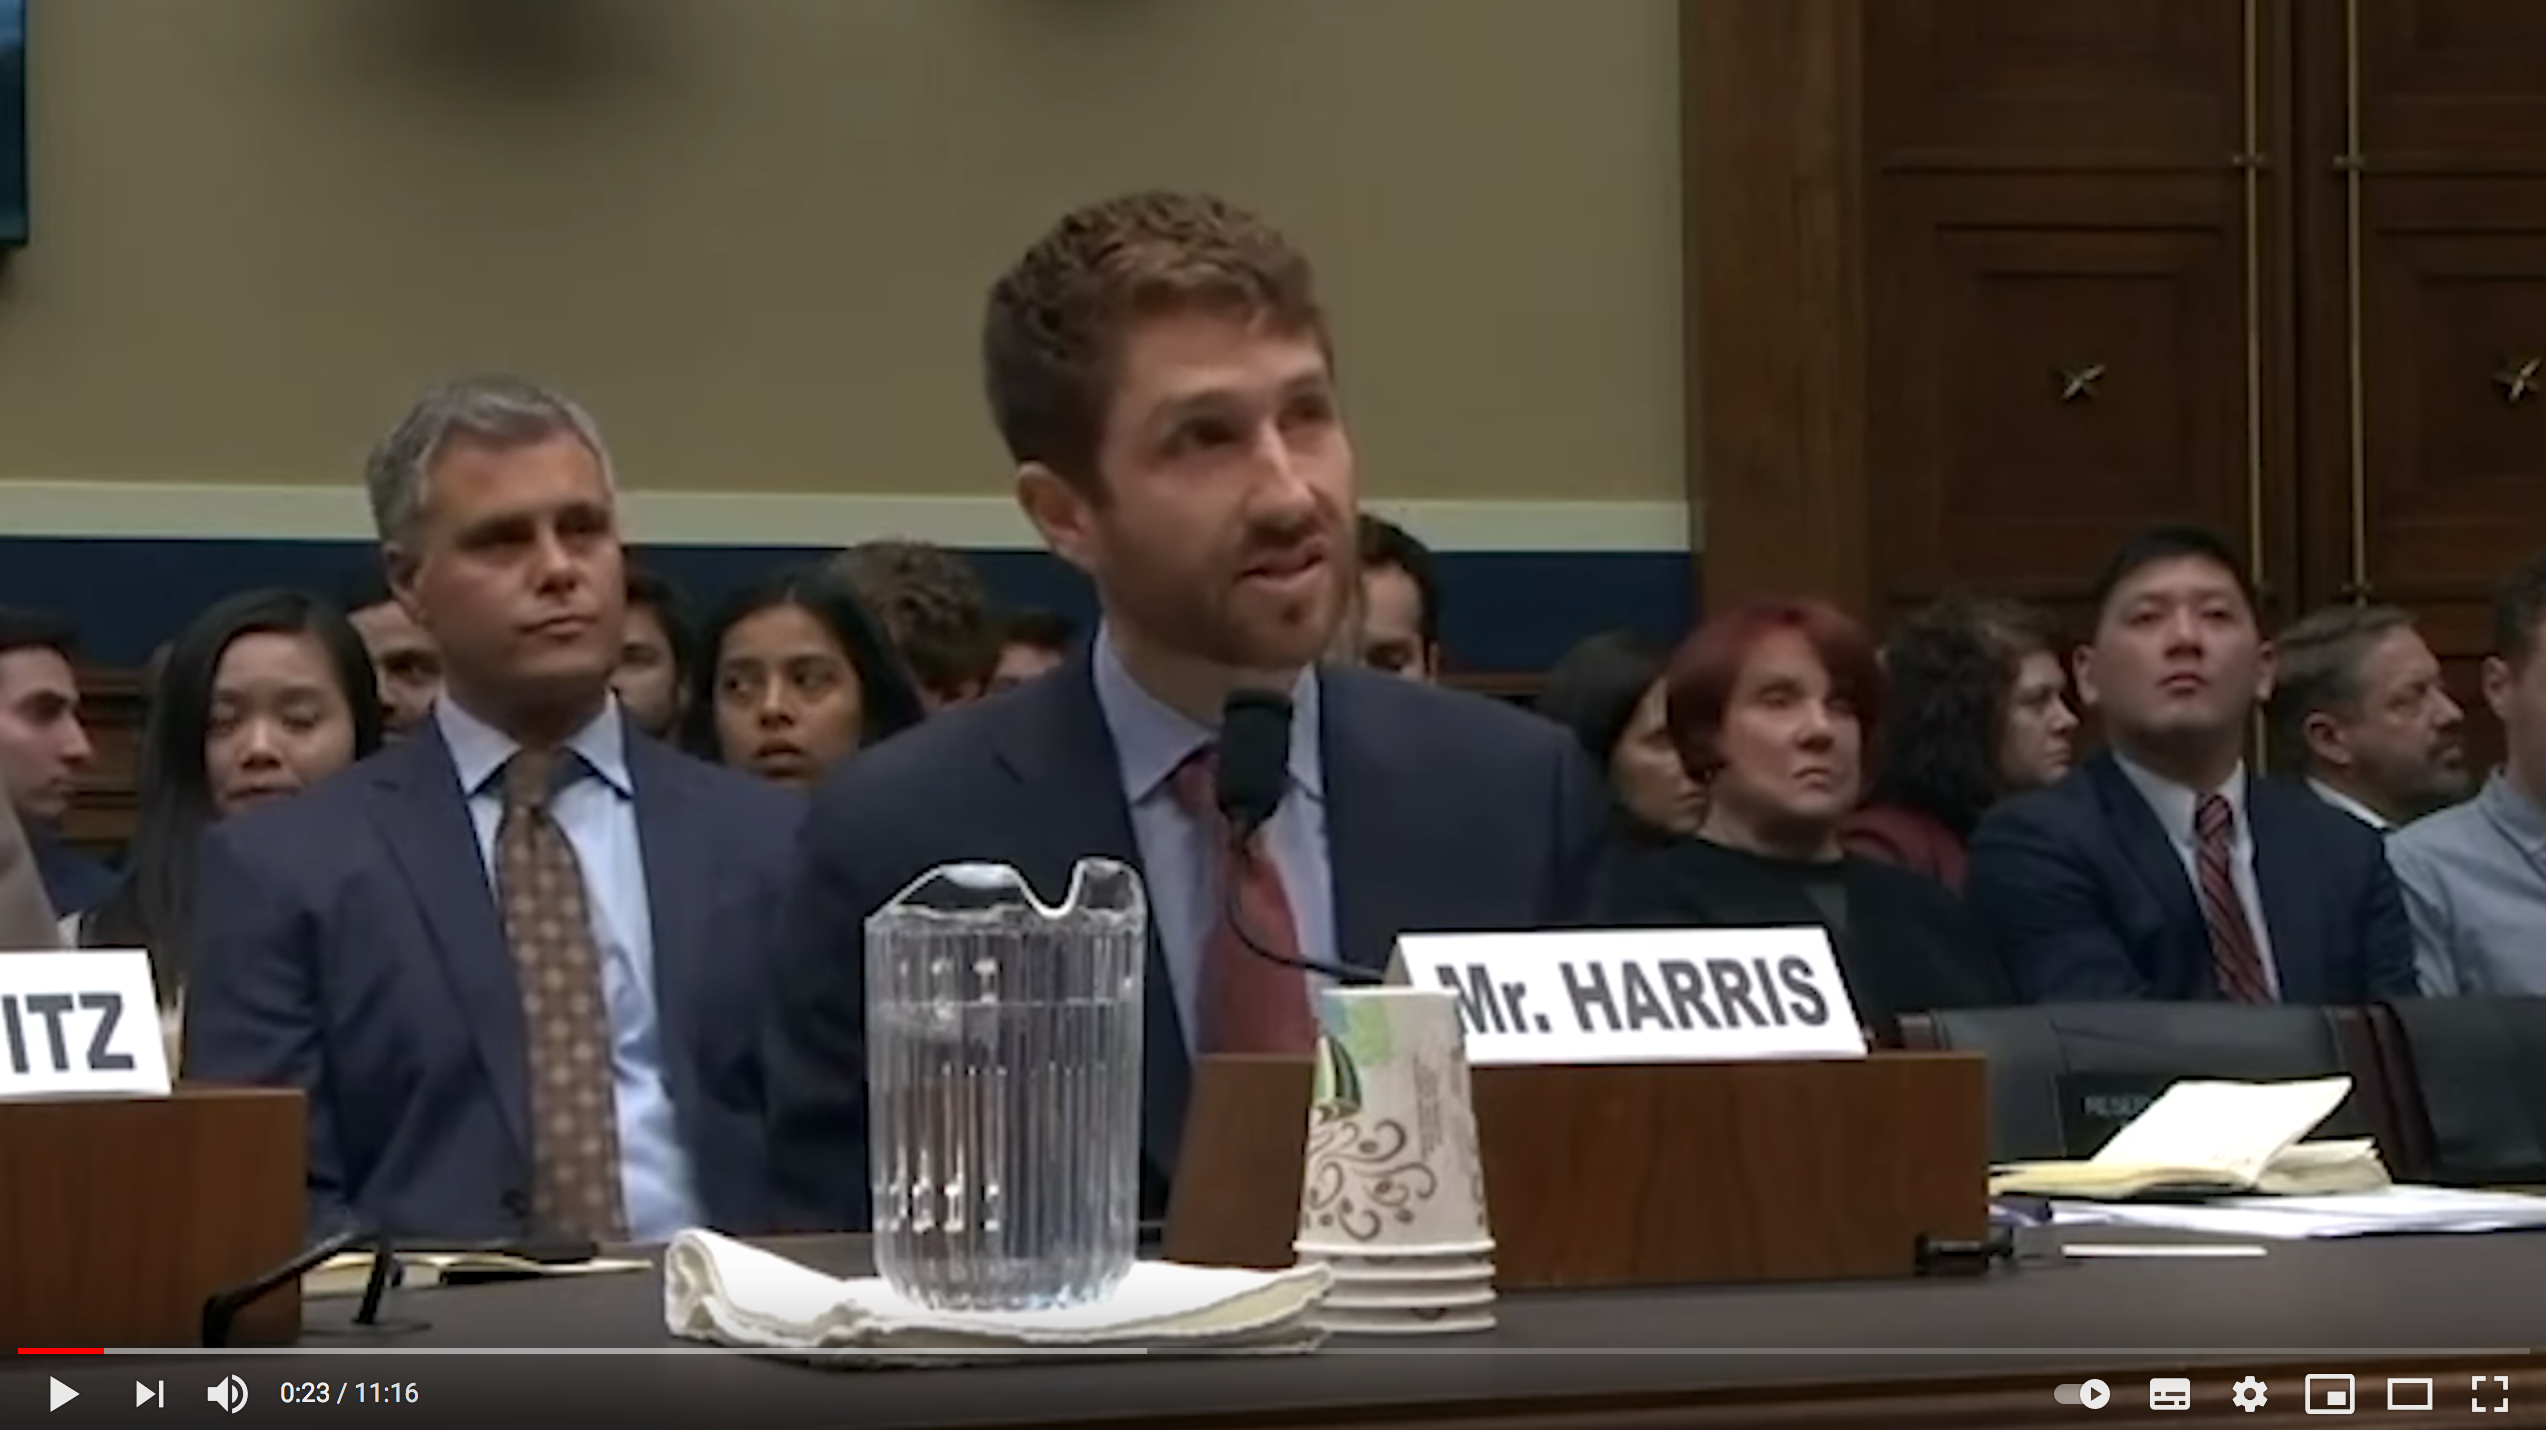
\includegraphics[width=\textwidth]{figures/harris_congress_2020}
\end{center}

\vfill

\url{https://www.youtube.com/watch?v=LUNErhONqCY}

\end{frame}
%%%%%%%%%%%%%%%%%%%%%%%%%
\begin{frame}

Two broad categories:  Structural changes vs tweaks

\note{
Tweaks might not make a big difference but we have a better chance of knowing what will happen
Unclear what will happen with structural change
}

\end{frame}
%%%%%%%%%%%%%%%%%%%%%%%%%%%
\begin{frame}

\begin{center}
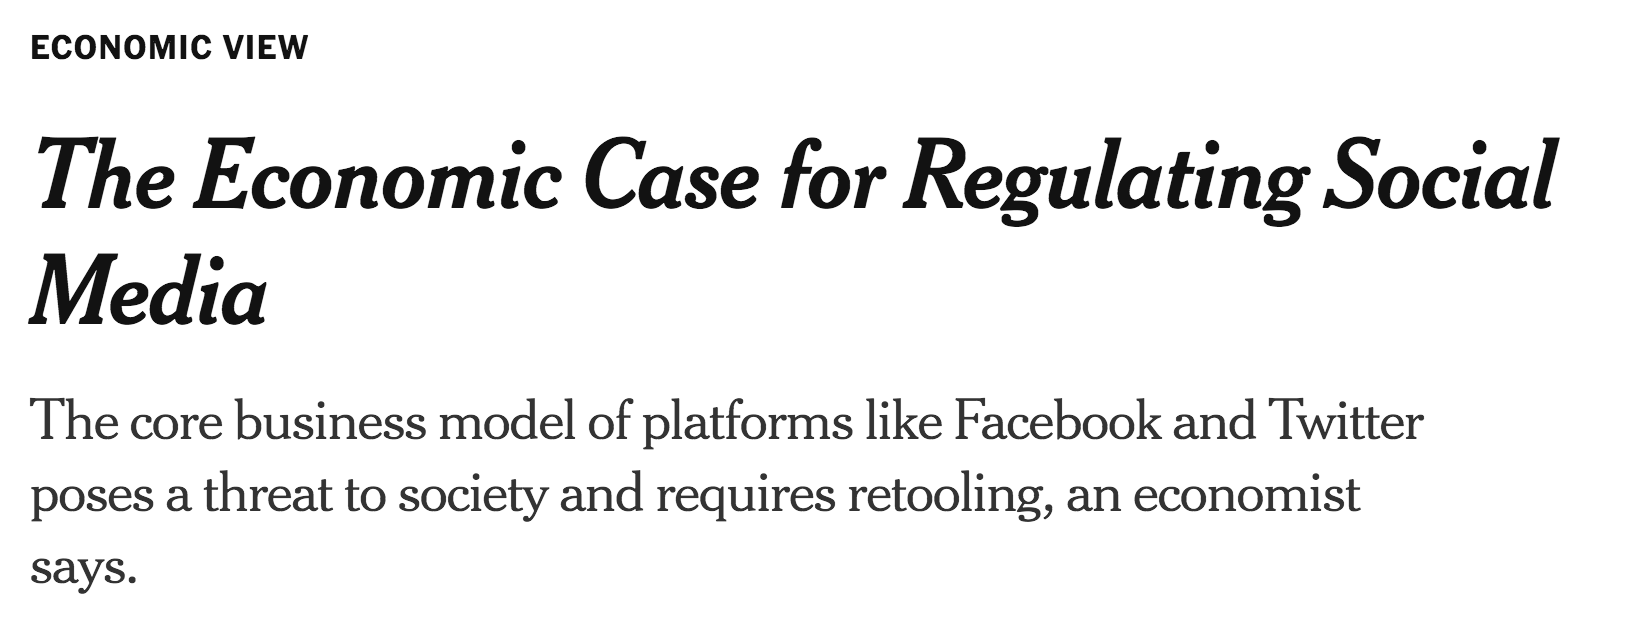
\includegraphics[width=0.8\textwidth]{figures/frank_economic_2021_headline}
\end{center}

Force social media companies to switch to a subscription model. \pause What kinds of changes would happen?  How can we know? Who would be harmed?

\end{frame}
%%%%%%%%%%%%%%%%%%%%%%%%%%%
\begin{frame}

Structural changes
\begin{itemize}
\item require subscriptions for social media \pause
\item creating online privacy regulations \pause
\item changing Section 230 of the Communications Decency Act (``No provider or user of an interactive computer service shall be treated as the publisher or speaker of any information provided by another information content provider'')
\end{itemize}

\end{frame}
%%%%%%%%%%%%%%%%%%%%%%%
\begin{frame}

\begin{center}
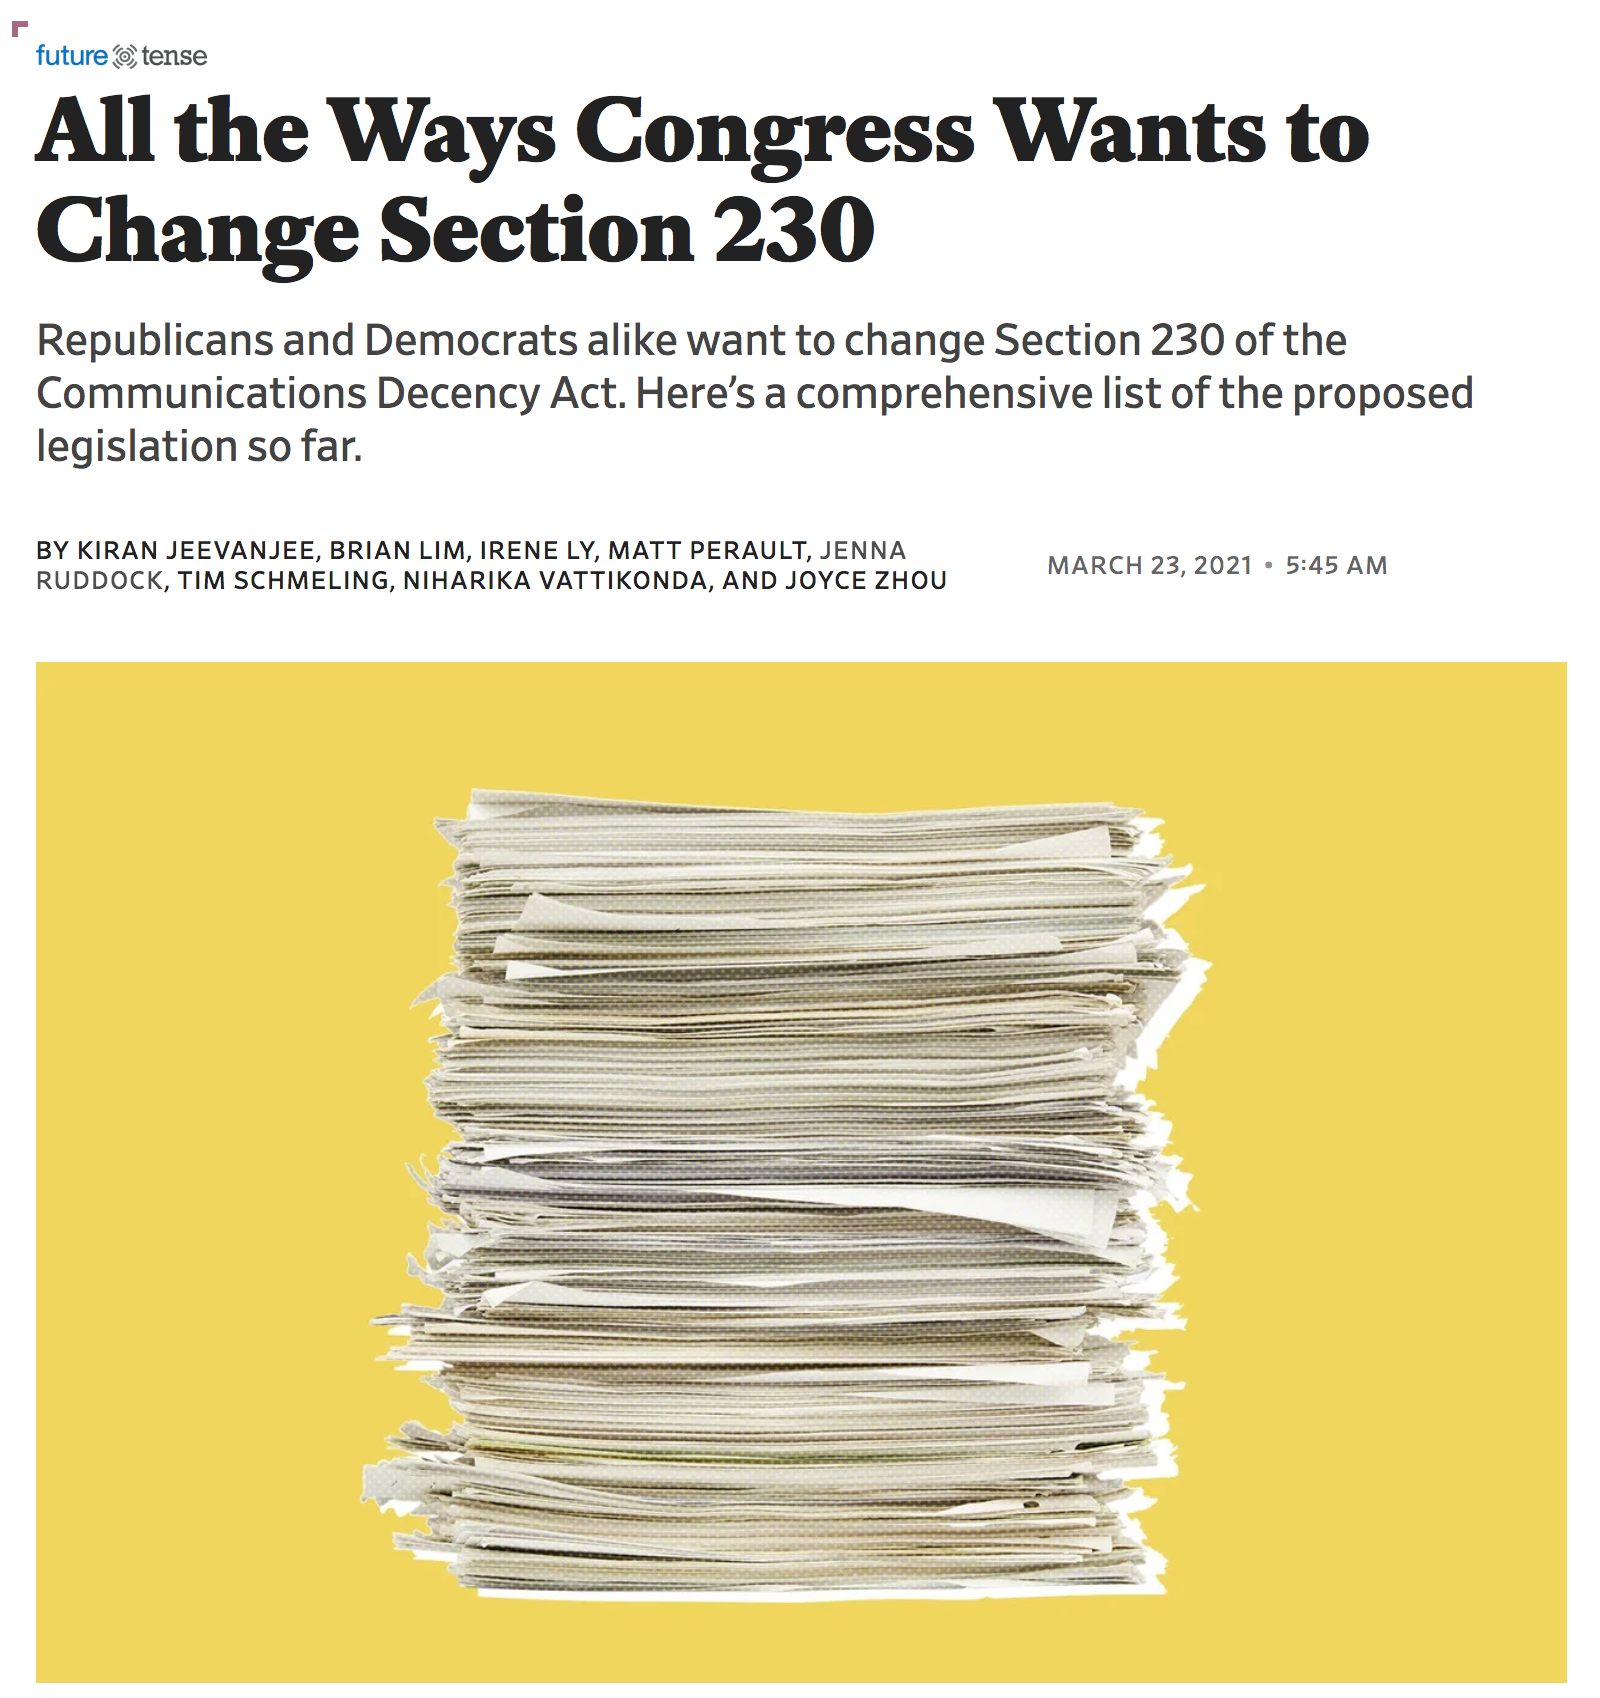
\includegraphics[width=0.5\textwidth]{figures/jeevanjee_all_2021_title}
\end{center}

\vfill
\url{https://slate.com/technology/2021/03/section-230-reform-legislative-tracker.html}

\end{frame}
%%%%%%%%%%%%%%%%%%%%%
\begin{frame}

\begin{itemize}
\item We don't know what impact any of these world have. \pause
\item This need require inaction but it should encourage humility.
\end{itemize}
\end{frame}
%%%%%%%%%%%%%%%%%%%%%
\begin{frame}

\begin{center}
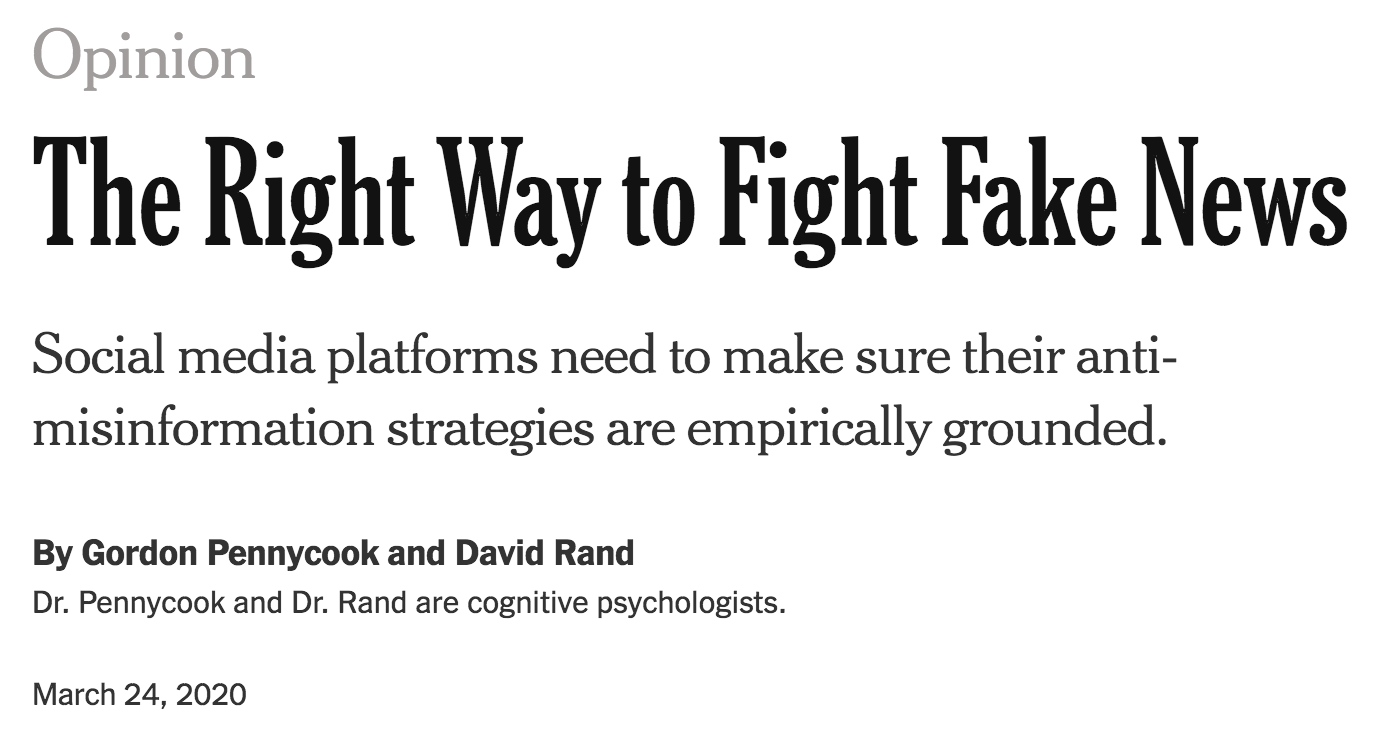
\includegraphics[width=0.4\textwidth]{figures/pennycook_right_2020_headline}
\end{center}

\begin{center}
\only<1>{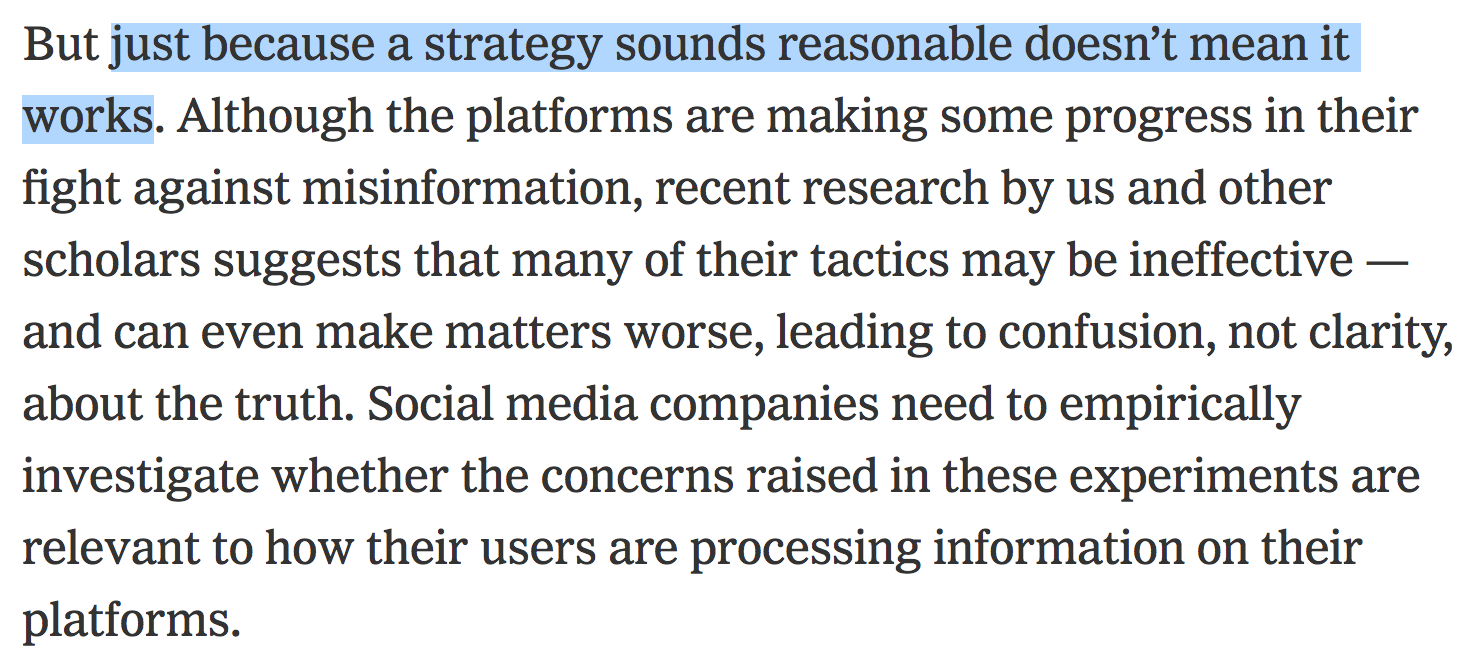
\includegraphics[width=0.6\textwidth]{figures/pennycook_right_2020_pullquote1}}%
\only<2>{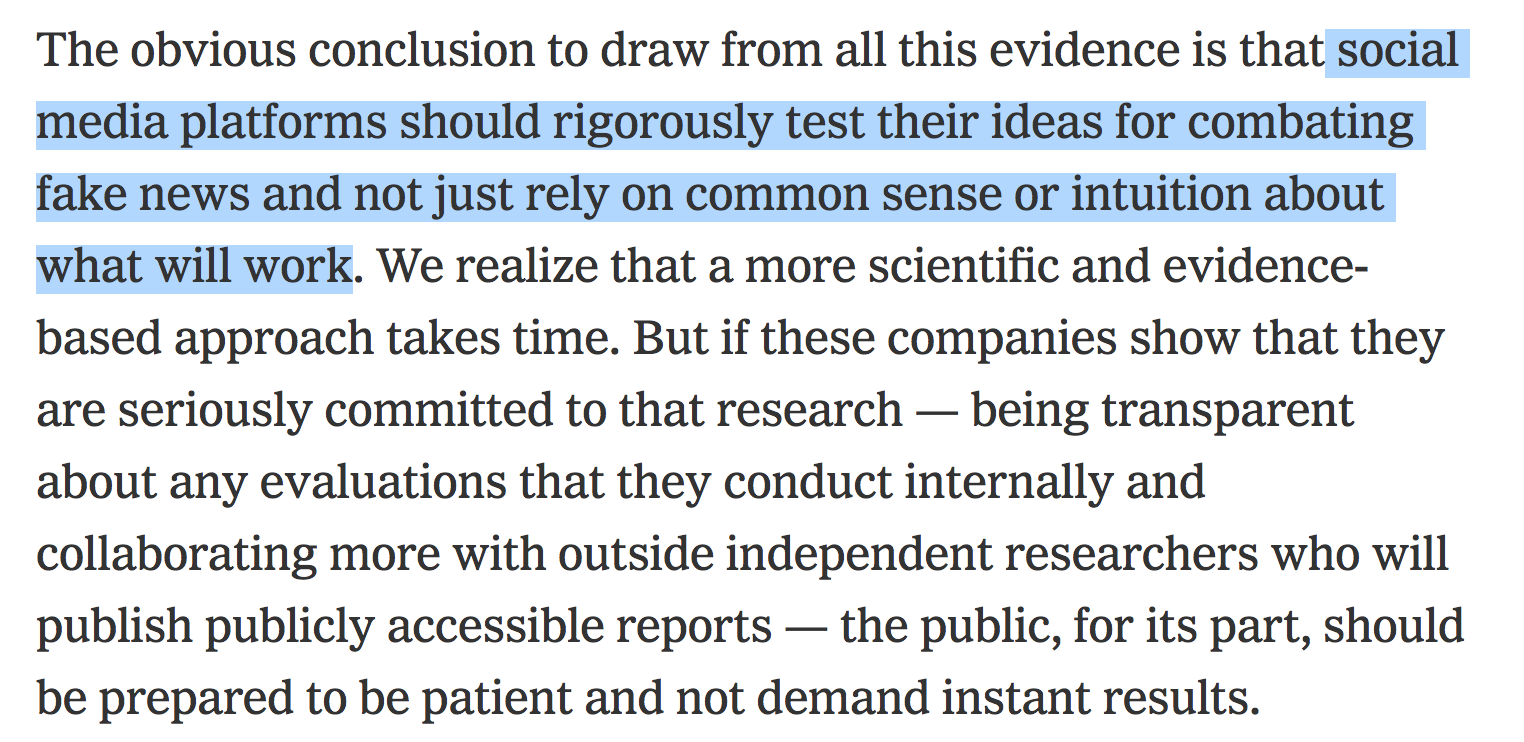
\includegraphics[width=0.6\textwidth]{figures/pennycook_right_2020_pullquote2}}%
\end{center}

\end{frame}
%%%%%%%%%%%%%%%%%%%%%
\begin{frame}

\begin{columns}

\begin{column}{0.5\textwidth}
\begin{center}
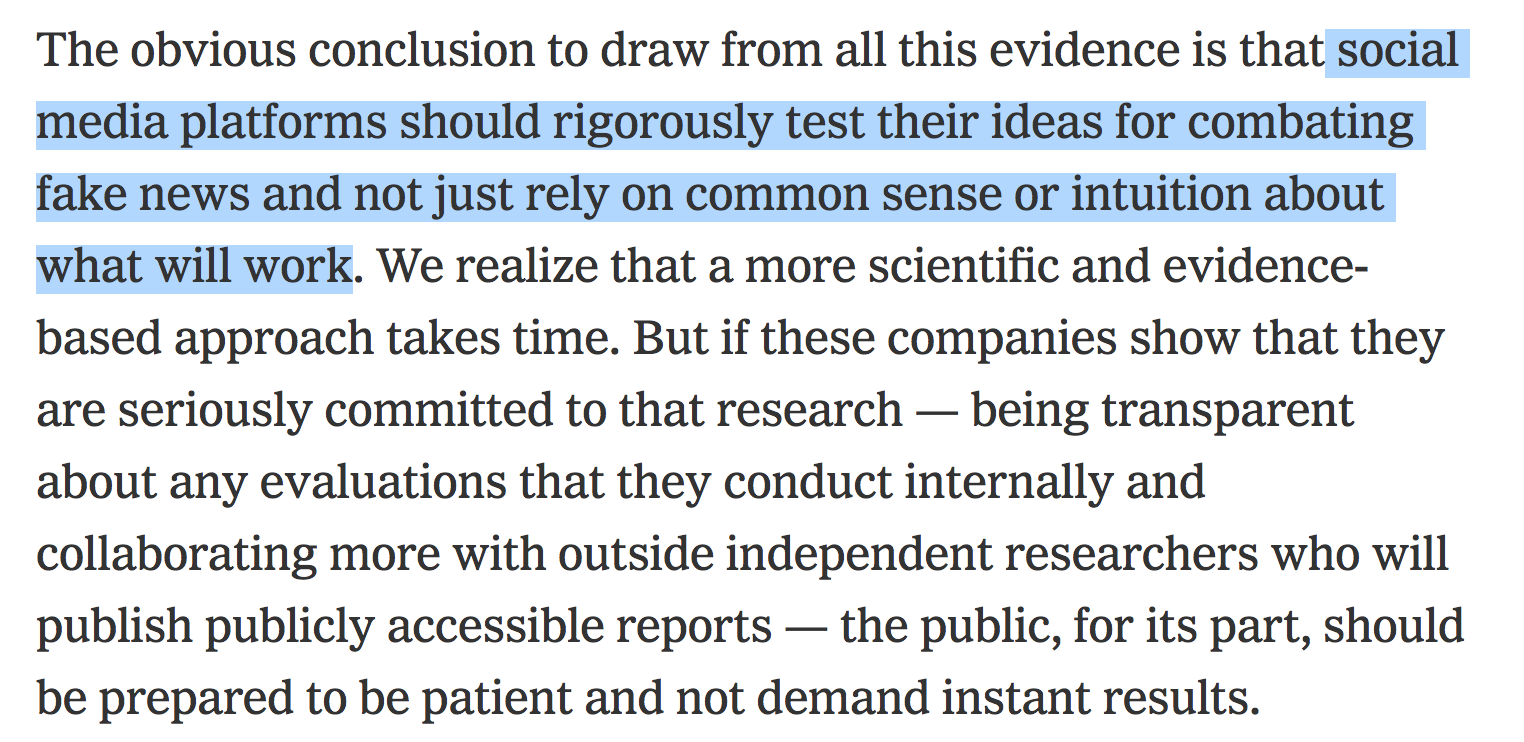
\includegraphics[width=0.8\textwidth]{figures/pennycook_right_2020_pullquote2}
\end{center}
\end{column}

\begin{column}{0.5\textwidth}
\begin{center}
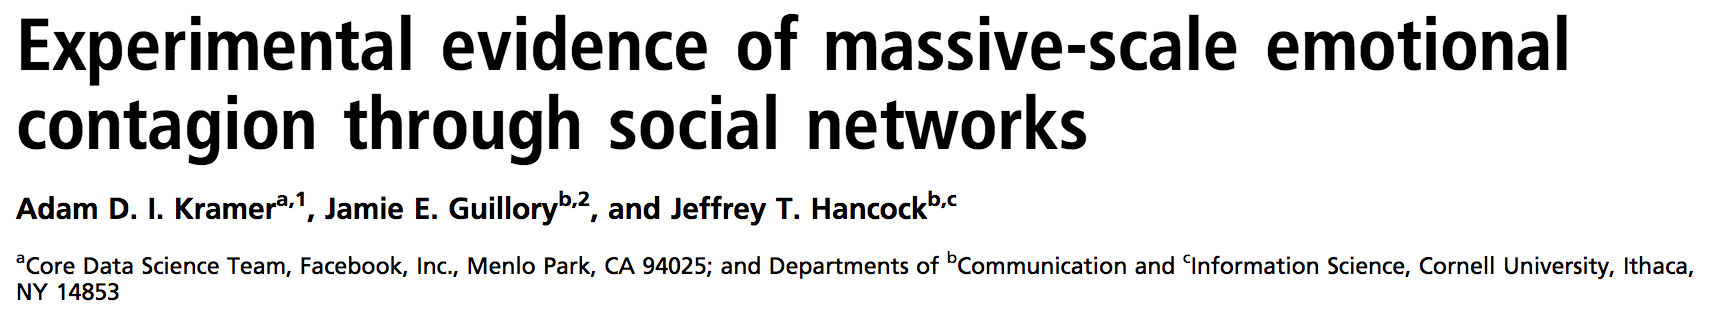
\includegraphics[width=0.8\textwidth]{figures/kramer_experimental_2014_title}
\end{center}
\end{column}

\end{columns}

\end{frame}
%%%%%%%%%%%%%%%%%%%%%
\begin{frame}

Let's see some interventions that can be tested

\end{frame}

\end{document}
